\documentclass[border=1mm]{standalone}

\usepackage{graphicx,tikz,tikz-layers}
\usetikzlibrary{decorations.markings,calc,positioning,arrows.meta}
% COLORS
\usepackage{xcolor}
\colorlet{myred}{red!80!black}
\colorlet{myblue}{blue!80!black}
\colorlet{mybluee}{myblue!80!black}
\colorlet{mygreen}{green!60!black}
\colorlet{myorange}{orange!70!red!60!black}
\colorlet{mydarkred}{red!30!black}
\colorlet{mydarkblue}{blue!40!black}
\colorlet{mydarkgreen}{green!30!black}

\begin{document}

\begin{tikzpicture}[
    font=\footnotesize,
    box/.style={draw, minimum width=3cm, minimum height=0.7cm, fill=myblue!15, rounded corners=3pt},
    patch/.style={minimum size=0.5cm},
    patch2/.style={minimum size=0.3cm},
    >={Latex[length=1.5mm, width=1.25mm]}
]

% Masked Image
\node[minimum size=2cm] (orig) at (0,0) {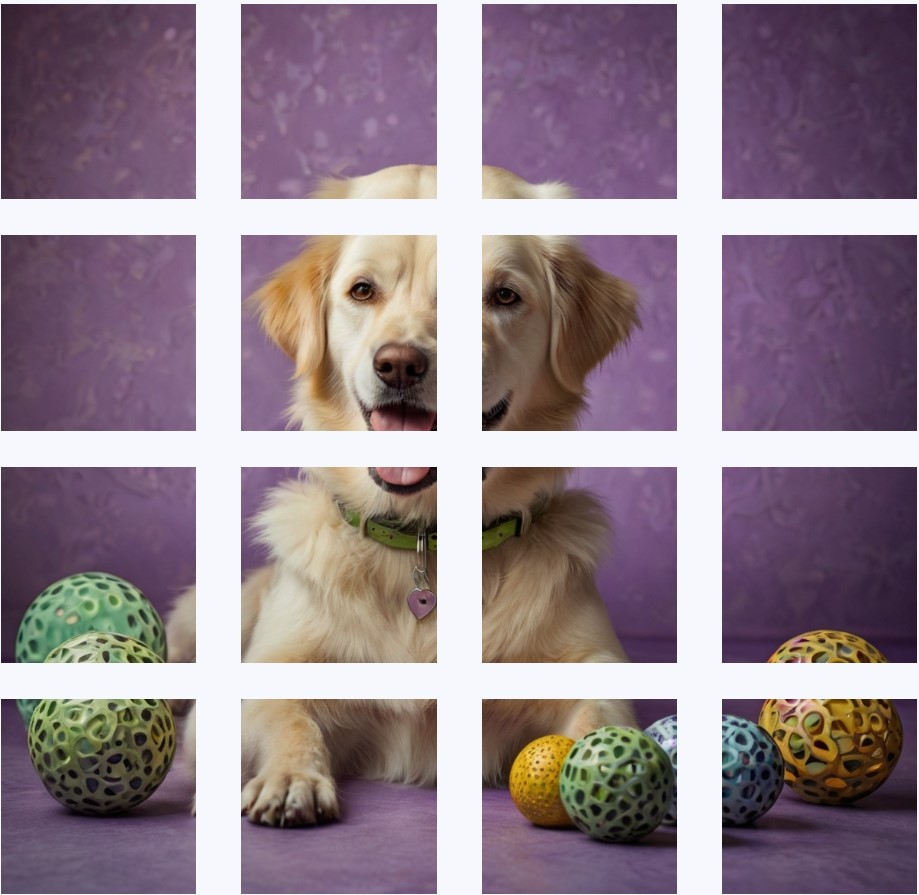
\includegraphics[width=2cm]{images/mosaic2/pdog.jpg}};
\node[fill=gray!50, draw,rectangle,minimum size=4.2mm, draw=gray!50, xshift =-0.26cm, yshift=0.25cm] {};
\node[fill=gray!50, draw,rectangle,minimum size=4.2mm, draw=gray!50, xshift =-0.26cm, yshift=0.75cm] {};
\node[fill=gray!50, draw,rectangle,minimum size=4.2mm, draw=gray!50, xshift =-0.26cm, yshift=-0.76cm] {};
\node[fill=gray!50, draw,rectangle,minimum size=4.2mm, draw=gray!50, xshift =0.78cm, yshift=0.25cm] {};
\node[fill=gray!50, draw,rectangle,minimum size=4.2mm, draw=gray!50, xshift =-0.78cm, yshift=-7.22] {};
\node[fill=gray!50, draw,rectangle,minimum size=4.2mm, draw=gray!50, xshift =0.78cm, yshift=0.75cm] {};
\node[fill=gray!50, draw,rectangle,minimum size=4.2mm, draw=gray!50, xshift =0.26cm, yshift=0.75cm] {};
\node[fill=gray!50, draw,rectangle,minimum size=4.2mm, draw=gray!50, xshift =0.78cm, yshift=-0.26cm] {};

\node[below=-0.02cm of orig] {Masked Image};

% Visible Patches
\node[patch] (p1) at (-2.1,2.1) {
\includegraphics[width=0.5cm]{tikz/images/mosaic2/00.jpg}};
\node[patch, right=-0.15cm of p1] (p2) {
\includegraphics[width=0.5cm]{tikz/images/mosaic2/01.jpg}};
\node[patch, right=-0.15cm of p2] (p3) {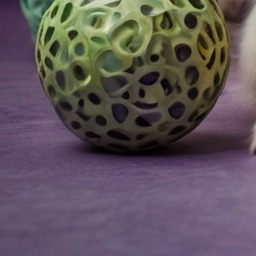
\includegraphics[width=0.5cm]{tikz/images/mosaic2/03.jpg}};
\node[patch, right=-0.15cm of p3] (p4) {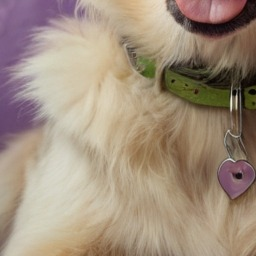
\includegraphics[width=0.5cm]{tikz/images/mosaic2/12.jpg}};
\node[patch, right=-0.15cm of p4] (p5) {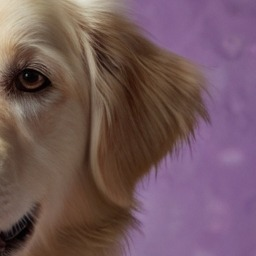
\includegraphics[width=0.5cm]{tikz/images/mosaic2/21.jpg}};
\node[patch, right=-0.15cm of p5] (p6) {
\includegraphics[width=0.5cm]{tikz/images/mosaic2/22.jpg}};
\node[patch, right=-0.15cm of p6] (p7) {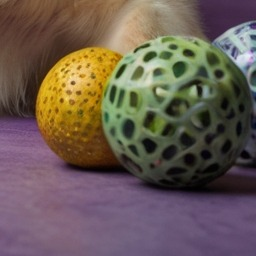
\includegraphics[width=0.5cm]{tikz/images/mosaic2/23.jpg}};
\node[patch, right=-0.15cm of p7] (p8) {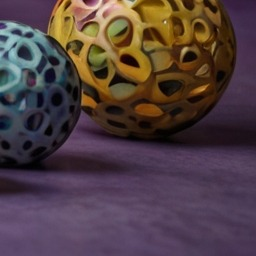
\includegraphics[width=0.5cm]{tikz/images/mosaic2/33.jpg}};

% \node at (3,1) {Visible Patches};

% Image Encoder
\node[box] (encoder) at (0,3.5) {Image Encoder};

% Text
\node[patch, fill=mybluee!20] (p1) at (4,2.1) {};
\node[patch, fill=mybluee!20, right=0.0851cm of p1] (p2) {};
\node[patch, fill=mybluee!20, right=0.0851cm of p2] (p3) {};
\node[patch, fill=mybluee!20, right=0.0851cm of p3] (p4) {};
\node[patch, fill=mybluee!20, right=0.0851cm of p4] (p5) {};

\node at (5.2,1.55) {Text};

% Text Encoder
\node[box] (textencoder) at (5.2,3.5) {Text Encoder};

% Contrastive Loss
\node[above=0.4cm of $(encoder.north)!0.5!(textencoder.north)$, align = center] (loss) {Contrastive \\ Loss};

% Arrows
\draw[->] (orig) -- ++(0,1.7);
\draw[->] (0,2.5) -- ++(0,0.5);
\draw[->] (5.2,2.5) -- ++(0,0.5);
% \draw[->] (p8) -- (encoder);
% \draw[->] (t6) -- (textencoder);
\draw[->] (encoder.north) -- ++(0,0.8) -- (loss.west);
\draw[->] (textencoder.north) -- ++(0,0.8) -- (loss.east);

\end{tikzpicture}

\end{document}